\documentclass[hyperref={pdfpagelabels=true}]{beamer}

\usepackage{lmodern}
%%%%%%%%%%%%%%%%%%%%%%%%%%%%%%%%%%%%%%%%%%%%%%%%%%%%%%%%%%%%%%%%%%%%%%%%%%%%%%%%%%%%%%%%%%%%%%%%%
%This work is licensed under a Creative Commons Attribution-ShareAlike 4.0 International License.
%
%You are free to:
%
%    Share — copy and redistribute the material in any medium or format
%    Adapt — remix, transform, and build upon the material
%    for any purpose, even commercially.
%
%    The licensor cannot revoke these freedoms as long as you follow the license terms.
%
%Attribution — You must give appropriate credit, provide a link to the license, and indicate if changes were made. You may do so in any reasonable manner, but not in any way that suggests the licensor endorses you or your use.
%
%ShareAlike — If you remix, transform, or build upon the material, you must distribute your contributions under the same license as the original. 
%
%%%%%%%%%%%%%%%%%%%%%%%%%%%%%%%%%%%%%%%%%%%%%%%%%%%%%%%%%%%%%%%%%%%%%%%%%%%%%%%%%%%%%%%%%%%%%%%%%
\definecolor{dred}{rgb}{0.647059, 0.164706, 0.164706}
\definecolor{dgreen}{rgb}{0., 0.545098, 0.545098}
\usecolortheme[named=dgreen]{structure}

\title{Visualizing Micro-blogging Data}
\subtitle{using Clustering and GIS}
\author{Joana Sim\~{o}es} 

\author[shortname]{Joana Sim\~{o}es \inst{1}}
\institute[shortinst]{\inst{1} Eurecat, Centre Tecnologic de Catalunya}

%\date{\today} 
%\titlegraphic{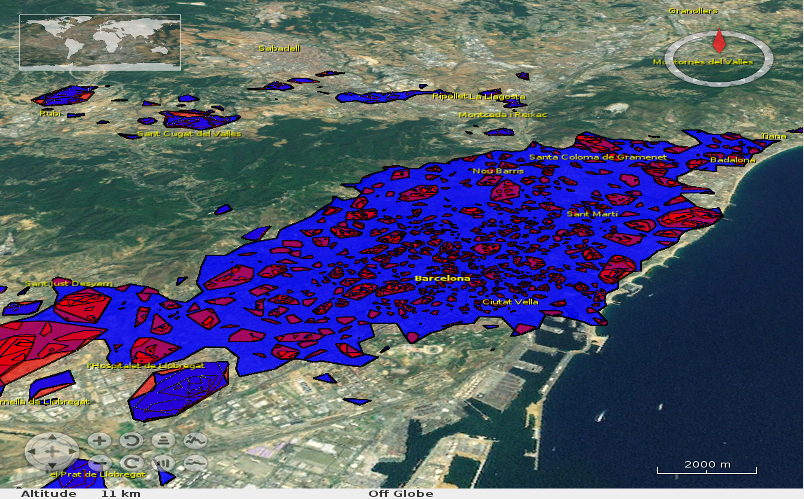
\includegraphics[width=.35\textwidth]{intro2.png}}
 
\usepackage{beamerthemeshadow}
%\usepackage{beamerthemesplit}
\usepackage{listings}

\newcommand{\soooo}{H$_2$SO$_4$}

%fdl stuff
\usepackage{hyperref}
\hypersetup{colorlinks, 
           citecolor=black,
           filecolor=black,
           linkcolor=black,
           urlcolor=black,
           bookmarksopen=true,
           pdftex}

\hfuzz = .6pt % avoid black boxes

\lstset{language=SQL}

\begin{document}
\setbeamertemplate{footline}[page number]
\setbeamertemplate{navigation symbols}{}
\begin{frame}
%\titlepage

\begin{titlepage}
\centering{ 
  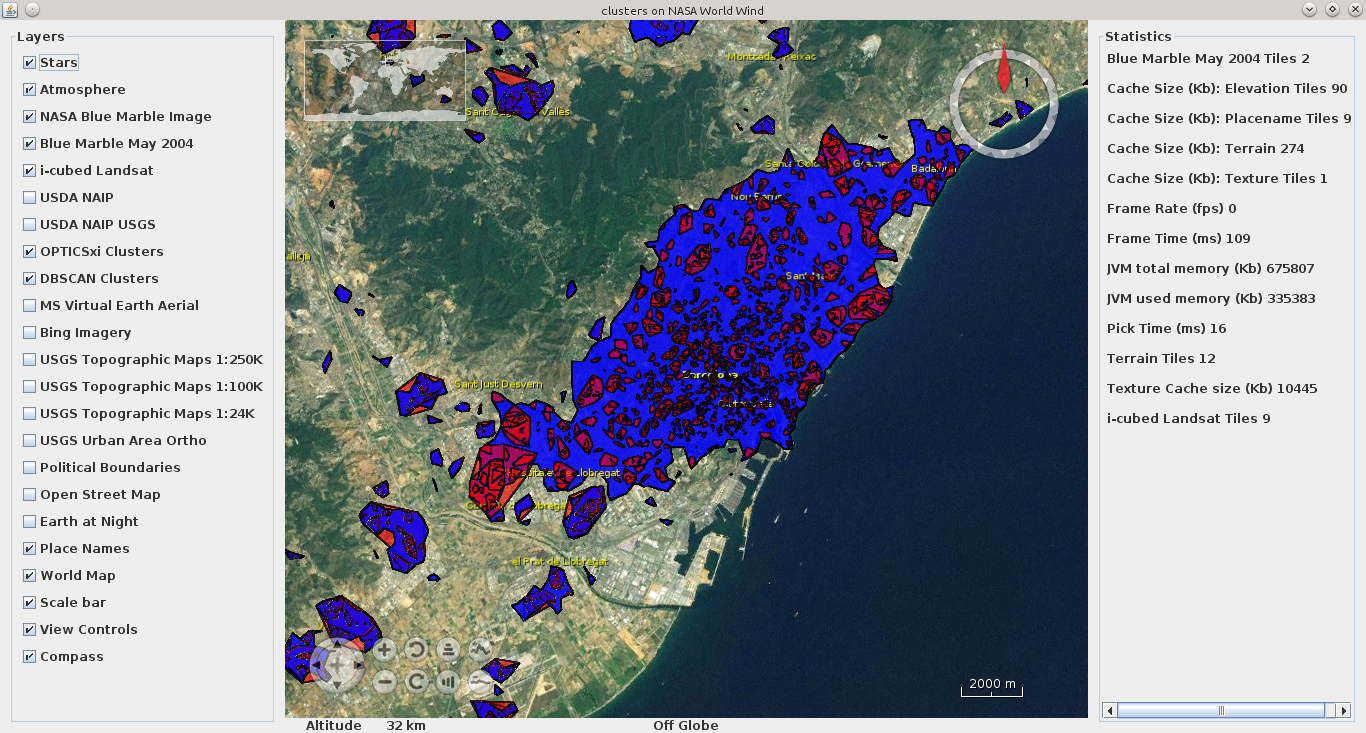
\includegraphics[scale=0.10]{screenshot1.png}
  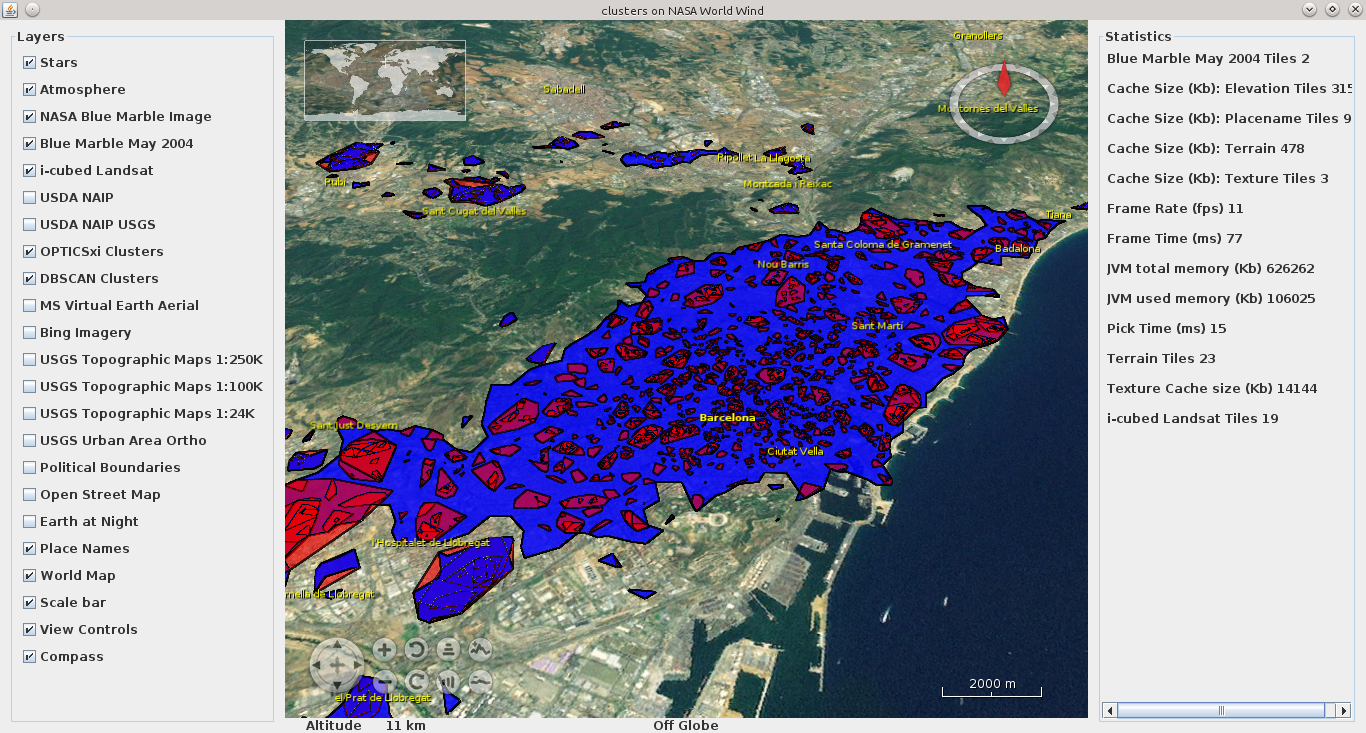
\includegraphics[scale=0.10]{screenshot3.png}
  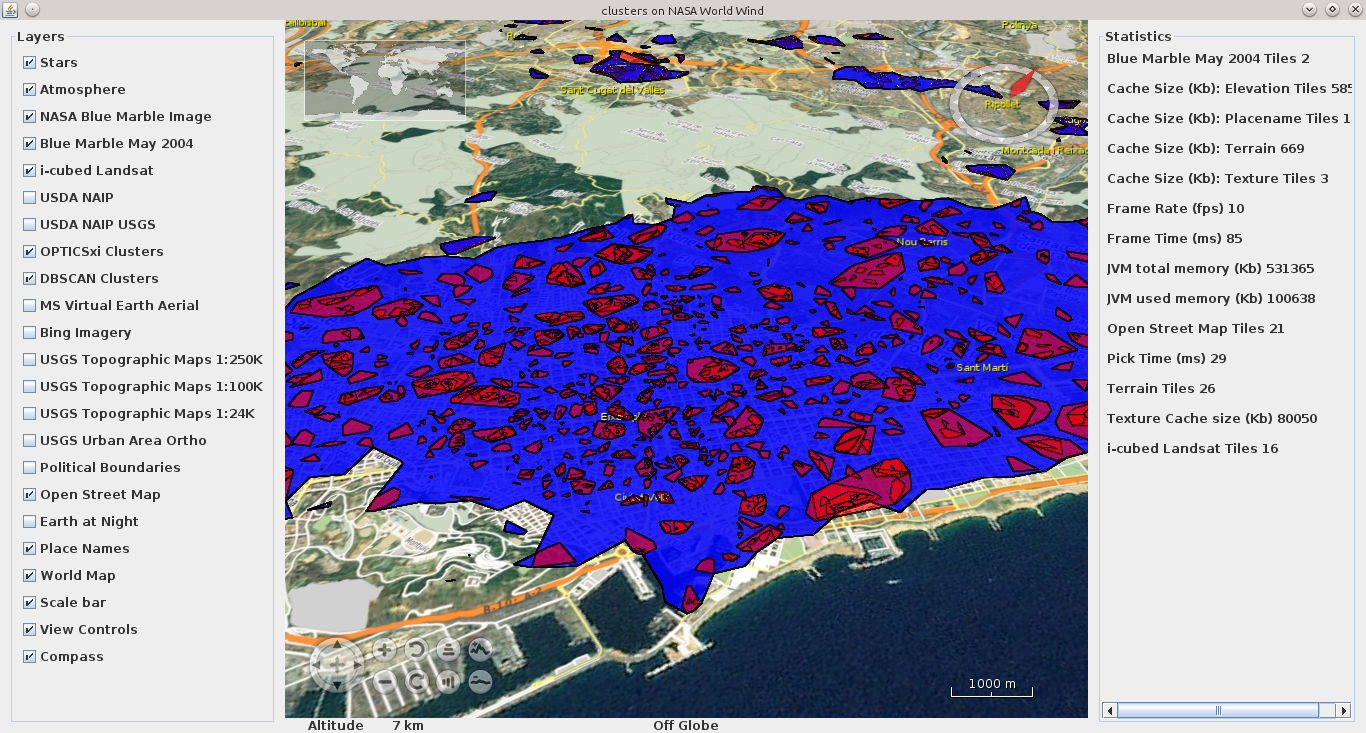
\includegraphics[scale=0.10]{screenshot4.png}  
}
\end{titlepage}

\end{frame} 
  
\begin{frame}
\frametitle{Table of Contents}
%\tiny{
\tableofcontents%}
\end{frame}

\section{Introduction} 
\begin{frame}
\frametitle{Introduction}
%TODO
%Ubiquitous computing and human-centric applications generate unprecedented records of human activity, with a very fine spatial and temporal resolution. To support the exploitation of micro-blogging data as an insight into the city’s activity, we devised an application that combines both, machine learning and Geographic Information Systems in a single interface.
\begin{columns}
  \begin{column}{0.7\textwidth}\small{ 

  \begin{itemize}    
    \item<1->Nowadays social media is a major source for information sharing. %In some cases the user also shares some attributes, such as \textbf{geolocation}. By using this information as a proxy for human presence
    \item<2->A proxy for human presence: powerful representations of the distribution of social media users within the territory.
    \item<3->Due to its willingness in sharing data, Twitter has been a prime \textit{playground}, for researchers and practitioners around the world.  
  \end{itemize} }
  \end{column}
  \begin{column}{0.3\textwidth}        
    \begin{figure}   
      
\includegraphics[width=\textwidth]{love.jpg}   
    \end{figure}     
  \end{column}  
\end{columns}    
\end{frame}

\begin{frame}
\frametitle{Twitter}
%TODO:what is Twitter
\begin{itemize}    
      \item<1->Users on Twitter generate over 400 million tweets everyday.%1 year BCN > 1 million records
      \item<2->Approximately 1\% of all Tweets published on Twitter are geolocated.
      \item<3->This amount of data is not easily assimilated by the "human-eye"
\end{itemize}          
  \begin{figure}   
    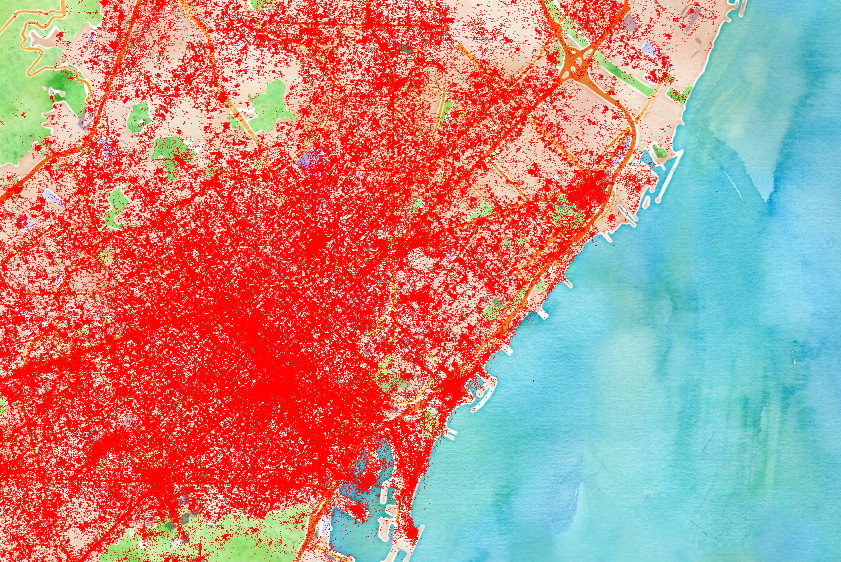
\includegraphics[width=0.4\textwidth]{bigdata1.png}   
  \end{figure}     
\end{frame}

\begin{frame}
\frametitle{Motivation}
\begin{columns}
  \begin{column}{0.5\textwidth}\small{ 
      How to assimilate these large datasets and extract some relevant information?
      \begin{itemize}    
	    \item<2->Technological Challenge + \textbf{Representation Challenge}
	    \item<3->Data mining/ Machine Learning      
      \end{itemize}                }
  \end{column}
  \begin{column}{0.5\textwidth}      
	\begin{figure}   
	  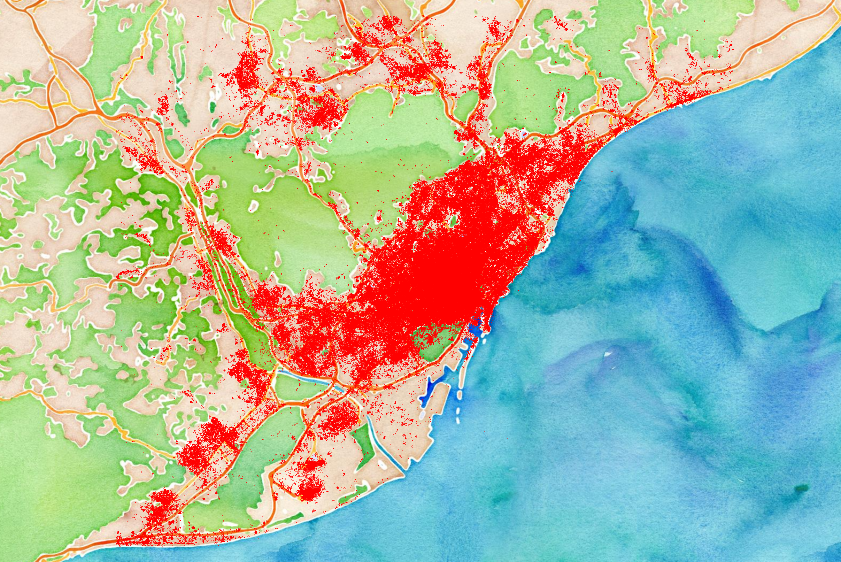
\includegraphics[width=\textwidth]{bigdata2.png}   
	\end{figure}     
  \end{column}  
\end{columns}
\end{frame}

\section{Extracting Patterns} 
\begin{frame}
\frametitle{Clustering}
%In order to summarize the dataset, we applied different clustering algorithms that have proved to complement each other by uncovering spatial patterns at multiple levels of detail.
\begin{columns}
  \begin{column}{0.5\textwidth}\small{ 
    \begin{itemize}
      \item<1->Widely used due to its segmentation and summarization features.
      \item<2->Unsupervised, descriptive, method.
      \item<3->Identifies groups of objects, which are similar between them, and distinct from the rest.
      %\item<3->It can be considered a concise model of the data, which can be interpreted in the sense of either a summary or a generative model 
      \end{itemize}  }
  \end{column}
  \begin{column}{0.5\textwidth}
      \begin{figure}  
	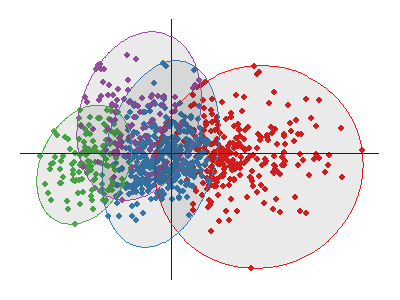
\includegraphics[width=0.8\textwidth]{Cluster_analysis.png}
       \end{figure}  
  \end{column}  
\end{columns}
\end{frame}

\begin{frame}
\frametitle{DBSCAN}
\begin{columns}
  \begin{column}{0.5\textwidth}\small{ 
    \begin{itemize}    
	  \item<2->Detects an a priori unknown, number of clusters with an arbitrary shape. %It implements a strict policy regarding what a
	  \item<3->Density-based clustering.% algorithm that 
	  \item<4->A \textit{dense-region} is defined by global parameters: 
	  \begin{itemize}
	    \item<5->epsilon: neighbourhood radius.
	    \item<5->minPts: minimum number of points required to form a dense region.
	  \end{itemize}                
    \end{itemize}              }  
  \end{column}
  \begin{column}{0.5\textwidth}    
      \begin{figure}   
	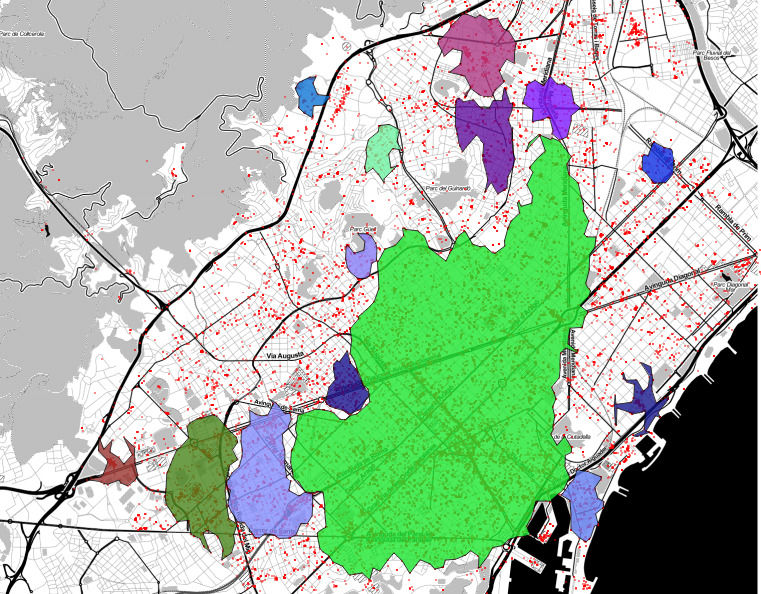
\includegraphics[width=\textwidth]{elki_dbscan_003_250.png}   
      \end{figure}     
  \end{column}  
\end{columns}
\end{frame}

%This “policy” is also the main weakness of DBSCAN, as the global parameters don’t allow capturing different densities in datasets such as Twitter. 

\begin{frame}
\frametitle{The Bottleneck: Global Parameters}
\begin{columns}
  \begin{column}{0.5\textwidth}
    \begin{figure}  
	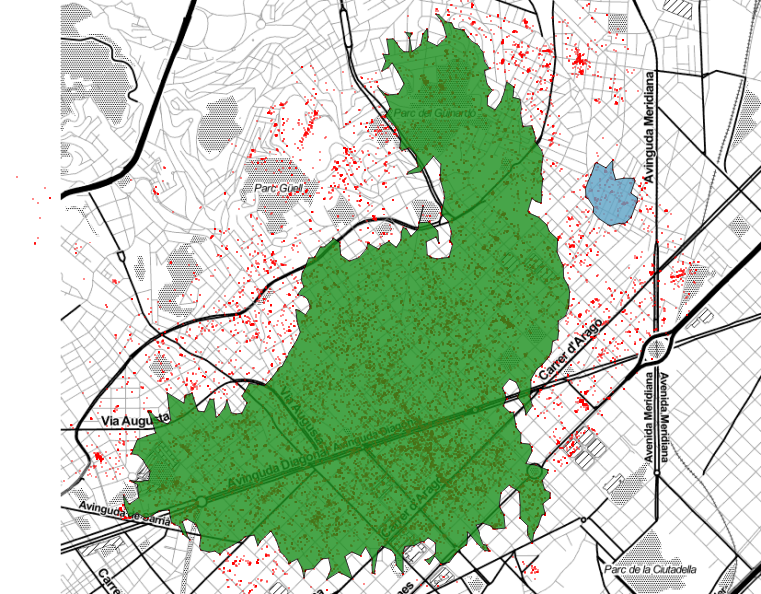
\includegraphics[width=\textwidth]{elki_dbscan_005_500.png}\\
           \tiny{Less strict combination of parameters}%higher epsilon and lower minpts  	          
       \end{figure}             
  \end{column}
  \begin{column}{0.5\textwidth}
      \begin{figure}  
	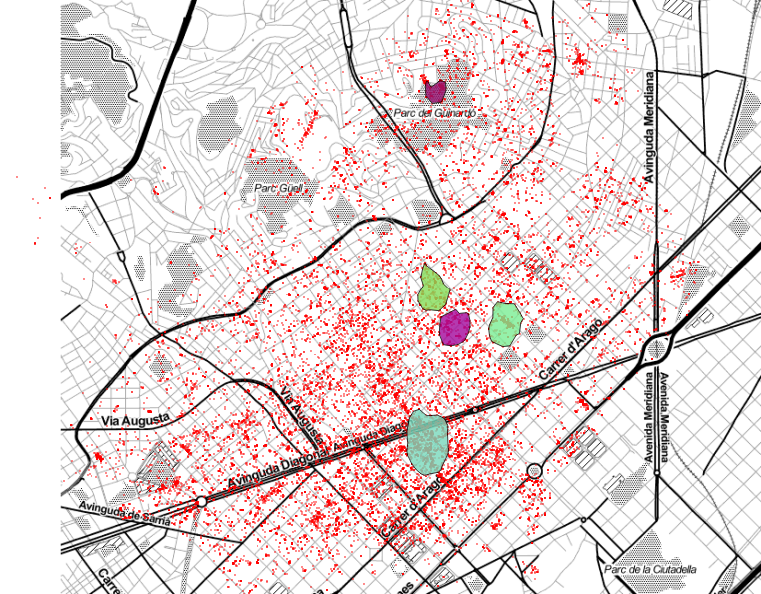
\includegraphics[width=\textwidth]{elki_dbscan_002_500.png}\\
           \tiny{Strict combination of parameters}%lower epsilon and higher minpts  	          
       \end{figure}  
  \end{column}  
\end{columns}
\end{frame}
% larger clusters that include a great part of the points, but it fails to expose the details of the highly dense zones, in the centre of the city; i.e.: we know that people gather in the city centre, but do they distribute uniformly within it, or concentrate more in certain areas such as squares or pedestrian roads? On the other hand, the “more strict” combination detects these zones, but leaves out other “potential” clusters that are less dense, in the city outskirts. 
%trade-off between detail and completness

%the fail to identify meaningful clusters in areas of varying density. A
\begin{frame}
\frametitle{OPTICS}
\begin{itemize}%It is considered a    
      \item<2->Generalization of DBSCAN.%, tackling its difficulty in configuring the parameters.%It is essentially an  
      \item<3->Ordering of the database, such as points that are spatially closest become neighbours in the ordering.
%This is represented in a diagram plotting this ordering and a special distance that is stored for each point, representing the density that needs to be accepted for a cluster in order to have both points belong to the same cluster.      
      \item<4->It does \textbf{not} produce a strict partition of the data.%, but it is possible to generate a clustering structure from the OPTICS output using another algorithm.     
\end{itemize}                
  \begin{figure}   
    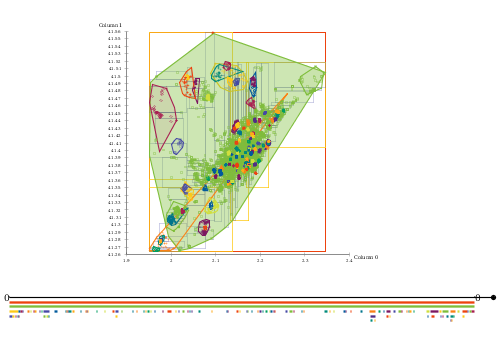
\includegraphics[width=0.55\textwidth]{optics_diag.png}   
  \end{figure}     
\end{frame}

\begin{frame}
\frametitle{Opticsxi: detecting Clusters}
\begin{itemize}
      \item<2->In the ordering clusters appear as \textit{valleys}, separated by \textit{noise regions}(peaks). 
      \item<3->We can define the \textit{start} and \textit{end} of a cluster, based on a threshold (xi).%Since "outer" clusters contain clusters with smaller reachability distances, The results of this partition will be hierarchical
      \item<4->Hierarchical partition.%more difficult to interpret, but it reveals something about teir structure.
\end{itemize}                
  \begin{figure}   
    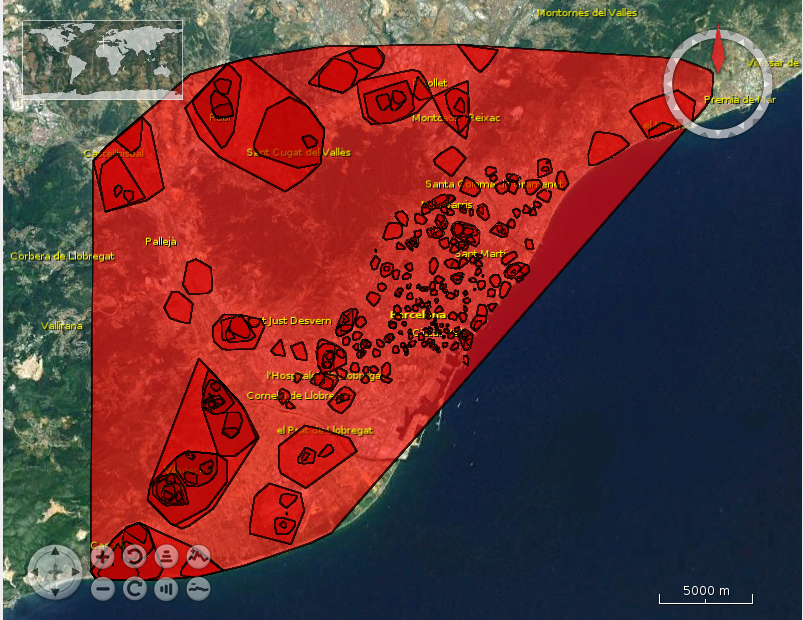
\includegraphics[width=0.5\textwidth]{2000_025_100_w_removal.png}   
  \end{figure}     
\end{frame}


\section{Putting Geographic Information into Context} 
\begin{frame}
\frametitle{GIS: Putting Geographic Information into Context}
    \begin{itemize}
      \item<1->Visualization is a key element to understand and interpret the results of data mining.%. In the case of a geospatial algorithm, it is particularly relevant to plot the results in a representation of the geographic space; i.e.: 
      \item<2->What about Geospatial information...?
      \item<3->WorldWind is an Open Source virtual globe developed by NASA that accesses a number of remote sensing datasets.%, including the Blue Marble Next Generation imagery, apart from other georeferenced images and geographic features served over the internet 
      \begin{itemize}
	  \item<3->OpenGL.%hardware accelerated rendering
       \end{itemize}
      \end{itemize}
      \begin{figure}  
	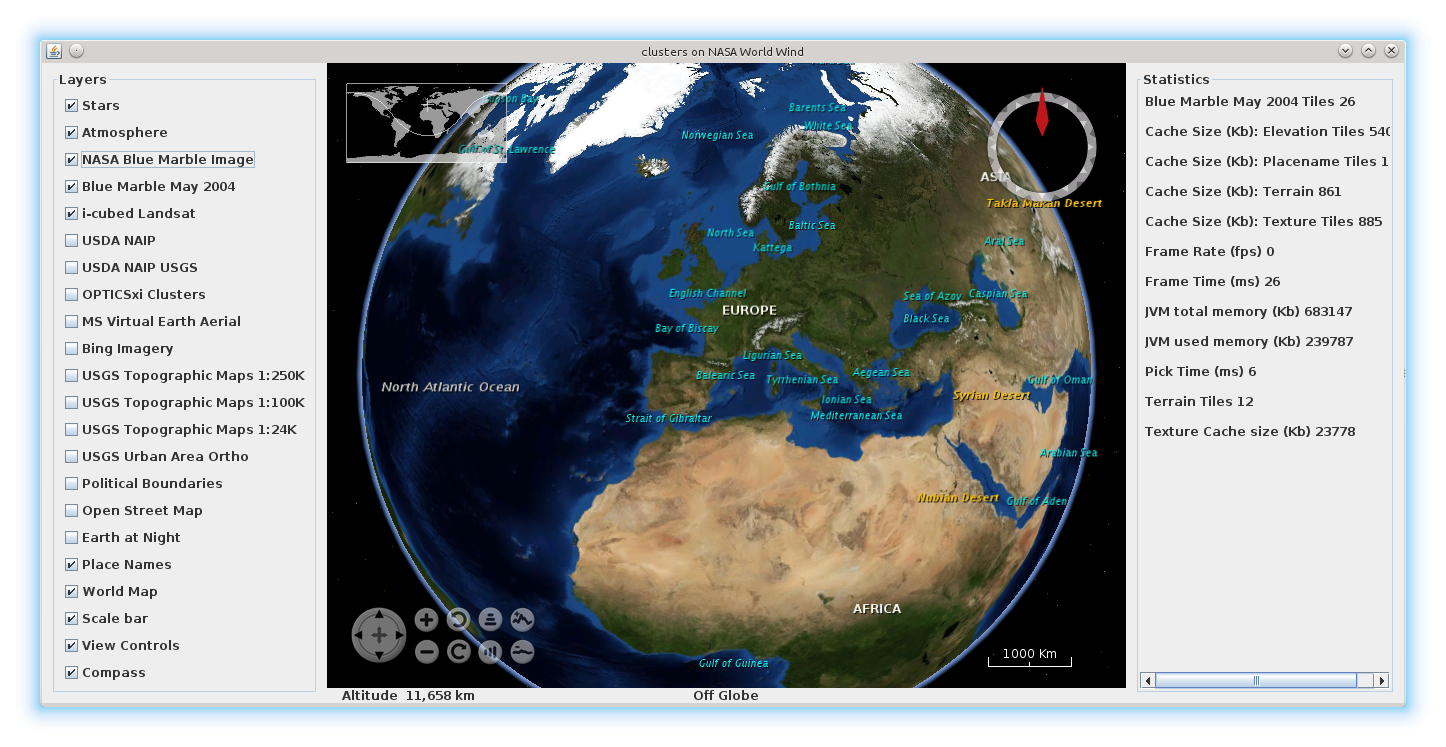
\includegraphics[width=0.7\textwidth]{bluemarble.png}
       \end{figure}  
\end{frame}

\begin{frame}
\frametitle{Cluster Explorer}
\begin{columns}
  \begin{column}{0.4\textwidth}
    \begin{itemize}
      \item<1->Java App based on FOSS.
      \item<2->Generates clusters based on DBSCAN, OPTICSxi (or both). 
      \item<3->Displays the results on a virtual globe.
      \end{itemize}      
  \end{column}
  \begin{column}{0.6\textwidth}      
      \begin{figure}  
	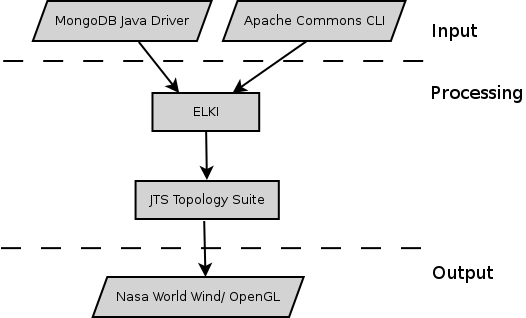
\includegraphics[width=\textwidth]{flowchart.png}
       \end{figure}  
  \end{column}       
\end{columns}  
\end{frame}

\section{A Case Study} 
\begin{frame}
\frametitle{A Case Study}
 A set of geo-located Tweets in the city of Barcelona, over a period of five days
\begin{columns}
  \begin{column}{0.5\textwidth}
    \begin{figure}  
	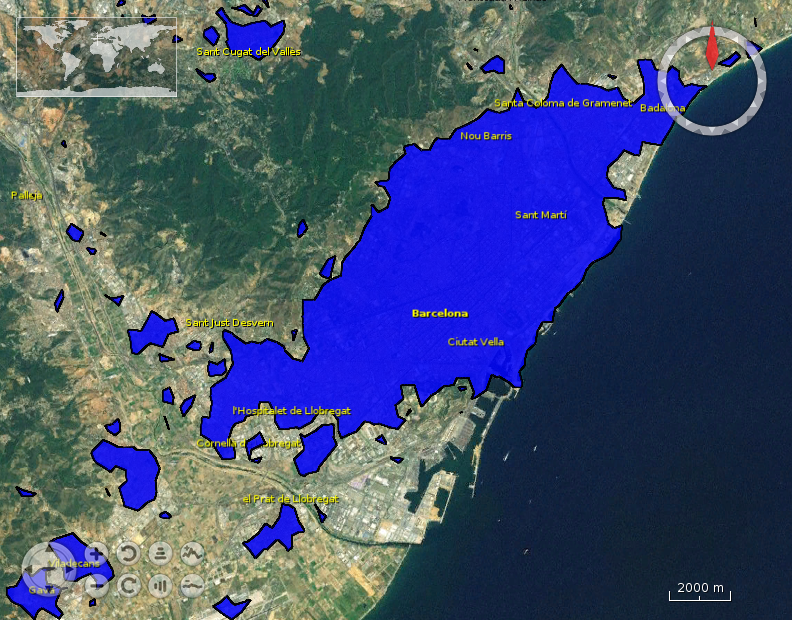
\includegraphics[width=\textwidth]{sim1b.png}\\
           \tiny{DBSCAN run}%lower epsilon and higher minpts  	    
       \end{figure}             
  \end{column}
  \begin{column}{0.5\textwidth}
      \begin{figure}  
	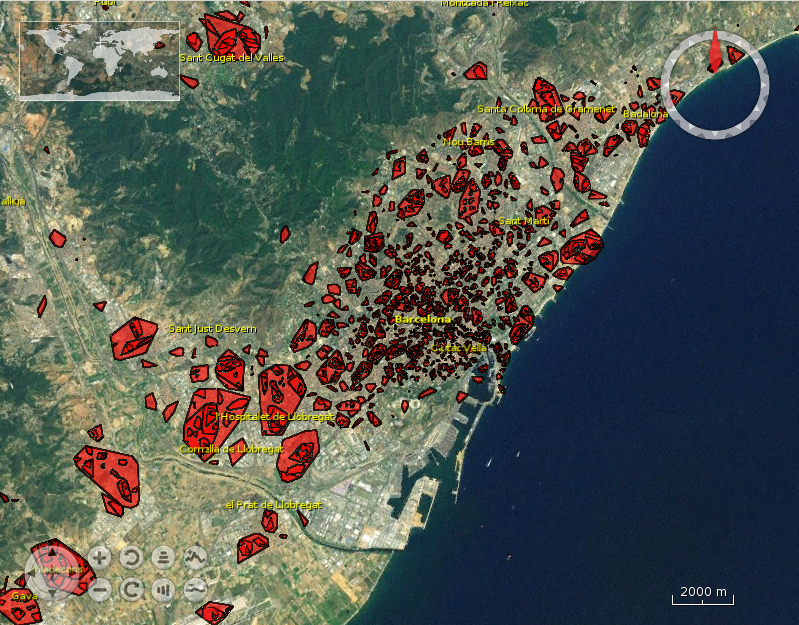
\includegraphics[width=\textwidth]{sim6.png}\\
           \tiny{OPTICSxi run}%higher epsilon and lower minpts  	      
       \end{figure}  
  \end{column}  
\end{columns}
%DBSCAN perceives central Barcelona as one single, large cluster, whether OPTICSXi detects many nested clusters within it, capturing local density changes.    
\end{frame}

\begin{frame}
\frametitle{GIS and the value of Location-Analysis}
%Plaza de Catalunya cluster. We identified that people gather in plaza catalunya, but since we are given an hierarchical structure, we can go further in our analysis and identify in which particular areas of Plaza Catalunya they concentrate more.
%Triangle - FNAC shop
%“Font de Canaletes”/Metro
%Hard rock cafe: tourists and tourist buses. Apart from being inside the café, people also tend to concentrate on its entrance, taking pictures, or just waiting for others in large groups. 
%Central gardens: there is the square itself, with its fountains and sculptures.
  \begin{figure}   
    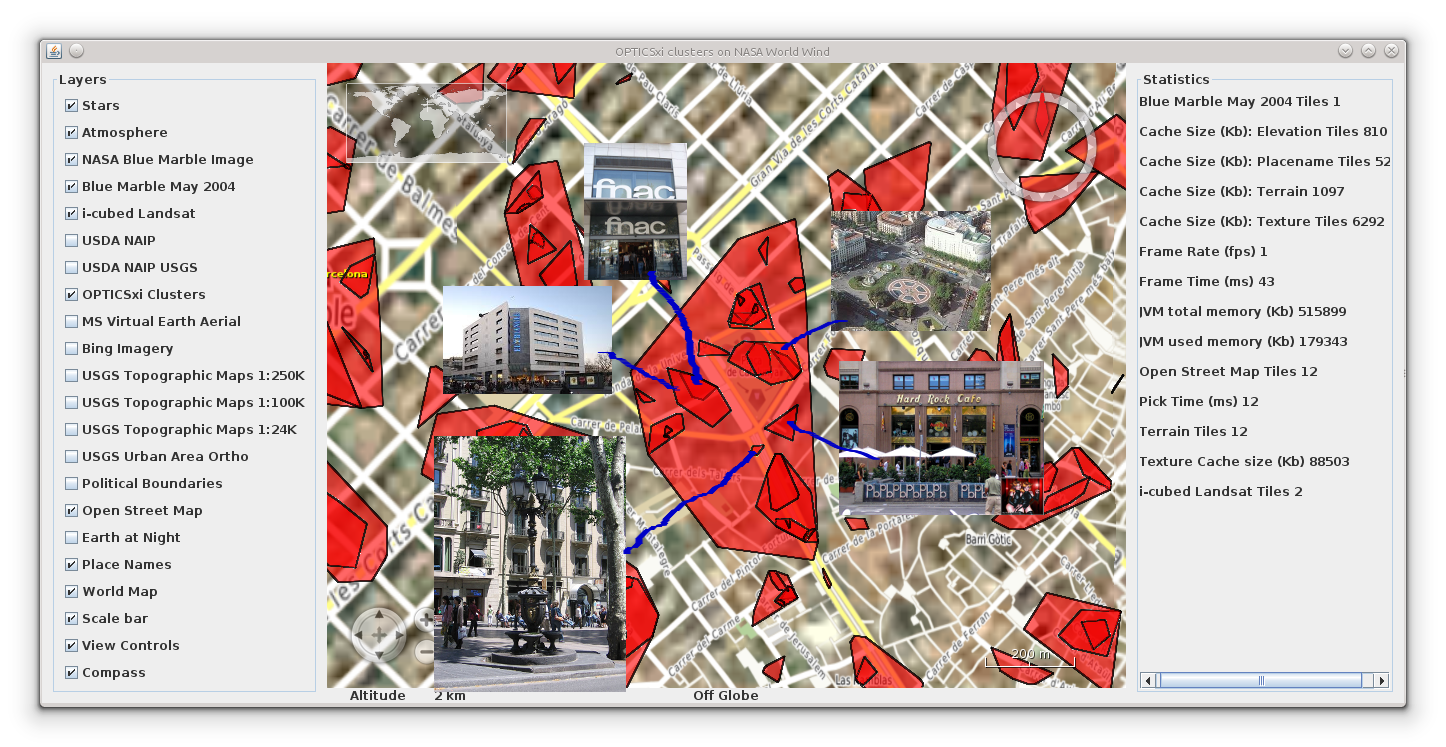
\includegraphics[width=\textwidth]{case_study.png}   
  \end{figure}     
\end{frame}


\section{Final Remarks}
\begin{frame}
\frametitle{Final Remarks}
    \begin{itemize}    
      \item<2->Flat cluster partition: summarizes the dataset and is easy to interpret.
      \item<3->Hierarchical cluster partition: allows to look at city at multiple scales.%Descending at the detail we want 
      \item<4->OPTICS: allows to detect clusters in areas of varying density.%overcoming this bottleneck of DBSCAN
      %\item<5->\textit{Cluster explorer}: effective for the exploration of micro-blogging data.
      \item<5->Visualizations provided by the use of a virtual globe have proved to be a flexible and context enhancing tool, that was crucial for the interpretation of the results.
      \item<6->We hope to have demonstrated some potentialities arising from the integration between spatial data mining and GIS technologies, using FOSS.   
     \end{itemize}
\end{frame}

\begin{frame}
\frametitle{Thank You!}
    \begin{figure}   
      
\includegraphics[width=0.4\textwidth]{thanks.jpg}      
    \end{figure}   
%    This presentation is available at: \centering{\\ \url{http://tinyurl.com/pcmgzxp}\\}
%      \vspace{5mm}    
\end{frame}

\end{document}